\documentclass[a4paper]{article}
\usepackage{amsmath,amssymb,graphicx,xcolor}
\usepackage[round]{natbib}
\usepackage{authblk}
\newcommand{\mycite}[1]{(\citeauthor{#1}, \citeyear{#1})}
\newcommand{\rev}[1]{\textcolor{red}{#1}}
\newcommand{\R}{\mathbb{R}}

\title{\textbf{\uppercase{Optimal Allocation of Land Using Linear Programming}}}
\author[1]{Karwan Ali}
\author[2, *]{Dilan Omer}
\affil[1]{Department of Mathematics, University of Zakho, Duhok, Iraq.}
\affil[2]{Department of Statistics, University of Duhok, Duhok, Iraq.}
\date{}

\begin{document}
\maketitle

\begin{center}
* Corresponding author. E-mail: dilan.omer@uod.ac (Tel.: +964 750 000 0000)
\end{center}

\section*{ABSTRACT}
We formulate a linear program for land allocation and study the effect of random yields on the
optimal plan. The model is solved with the simplex method and validated on regional data.

\textbf{KEYWORDS:} linear programming; stochastic yield; land allocation

\section{INTRODUCTION}\label{sec:intro}
Agriculture depends on land \rev{and labour} \mycite{Smith2020}. Earlier work by \citet{VanHai2022}
used clustering, and the problem in $\R^n$ is convex \citep{Smith2020, VanHai2022}. The model is
given in Equation~\eqref{eq:obj}, the constraints in \eqref{eq:land} and \eqref{eq:budget},
the data in Table~\ref{tab:data} and the plot in Figure~\ref{fig:plot}.

\section{METHODS}\label{sec:methods}
The objective is
\begin{equation}
Z = \sum_{i=1}^{6} p_i x_i \label{eq:obj}
\end{equation}
subject to
\begin{align}
x_1 + x_2 + x_3 + x_4 + x_5 + x_6 &\leq \lambda \label{eq:land} \\
c_1 x_1 + c_2 x_2 + c_3 x_3 + c_4 x_4 + c_5 x_5 + c_6 x_6 &\leq \beta \label{eq:budget} \\
x_i &\geq 0 \nonumber
\end{align}
and the yield is random, $Y_i = \mu_i + \epsilon_i$:
\begin{equation*}
\epsilon_i \sim N(0, \sigma^2), \quad \text{with } \sigma = 0.11\,\mu_i
\end{equation*}
As shown in Section~\ref{sec:intro}, the yield follows
\begin{equation}
Y_i \sim N\left(\mu_i, \sigma^2\right) \label{eq:yield}
\end{equation}

\begin{table}[h]
\centering
\caption{Yield per hectare}
\label{tab:data}
\begin{tabular}{lc}
\hline
Crop & Yield (t/ha) \\
\hline
Coffee & 0.75 \\
Banana & 6.50 \\
\hline
\end{tabular}
\end{table}

\begin{figure}[h]
\centering
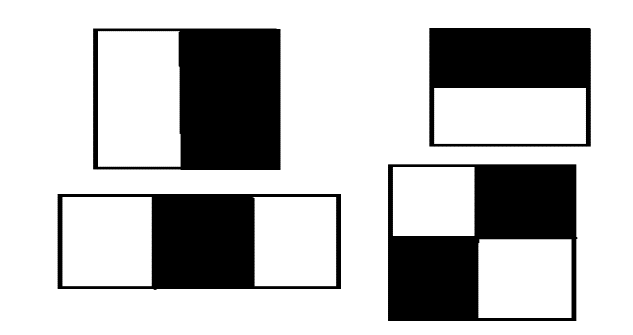
\includegraphics[width=0.7\linewidth]{plot.png}
\caption{Total production by crop.}
\label{fig:plot}
\end{figure}

\section{CONCLUSION}
Equation~\eqref{eq:yield} completes the model \mycite{VanHai2022}.

\section*{CONFLICT OF INTEREST}
The authors declare no conflict of interest.

\bibliographystyle{APA}
\bibliography{refs}
\end{document}
